\documentclass[a4paper,14pt]{article}         % класс документа - статья. Также report, book и др.
\usepackage{geometry}           % пакет для задания полей страницы командой \geometry
\geometry{a4paper, left=3cm,right=1.5cm,top=2cm,bottom=2cm}
%\usepackage[cp1251]{inputenc}   % кодировка текста
%\usepackage{mathtext}           % позволяет использовать русские буквы в формулах
%\usepackage[T2A]{fontenc}       %пакет Т2А необходим для правильного отображения кириллицы и переноса слов
%\inputencoding{cp1251}          % тоже кодировка...
\usepackage[utf8]{inputenc}
\usepackage[T2A]{fontenc}
\usepackage[russian]{babel}
%\usepackage{textcomp}
%\usepackage[unicode]{hyperref}  %создаёт гиперссылки на список литературы в pdf-файле
\usepackage{amstext,amsmath,amssymb}            % пакеты для формул
\usepackage{bm}                 % boldmath - пакет для жирного шрифта
\usepackage[pdftex]{graphicx}   % пакет для включения рисунков в форматах png,pdf,jpg,mps,tif
                                % надо компилировать сразу в pdf
\usepackage{hyperref}			% ссылки
\usepackage{amsfonts}           % греческие символы и, возможно, что-то ещё
\usepackage{indentfirst}        % одинаковый отступ для первого параграфа и всего остального
%\usepackage{cite}               % команда /cite{1,2,7,9} даёт ссылки
\usepackage{multirow}           % пакет для объединения строк в таблице: надо указать число строк и ширину столбца
\usepackage{array}              % нужен для создания таблиц
\linespread{1.3}                % полтора интервала. Если 1.6, то два интервала

% Подписи рисунков
\usepackage[font=Large,labelfont=bf]{caption}
\DeclareCaptionLabelSeparator{defffis}{ --- }
\captionsetup{justification   = raggedright,
			singlelinecheck = false,
			labelsep=defffis,}
\usepackage{subcaption}

% Шрифты секций
\usepackage{sectsty}
\sectionfont{\centering\fontsize{14}{15}\selectfont}
\subsectionfont{\fontsize{14}{15}\selectfont}
\subsubsectionfont{\fontsize{13}{15}\selectfont}

% Внутри секции картинки
\usepackage[section]{placeins}

% рекомендуется при использвоании biblatex
\usepackage{csquotes}
%\bibliographystyle{unsrt}
\bibliographystyle{ugost2008}

\usepackage[%
autolang=other,       
bibencoding=utf8,
sorting=none, % Name,Title,Year или sorting=none.
maxbibnames=4, % Максимальное число авторов в списке литературы.
minbibnames=2, % Число авторов, отображаемое при сокращении.
style=gost-numeric,
backend=biber]{biblatex}
\addbibresource{cite/Literature.bib}
%\bibliography{Literature.bib}
%
\if 0 \usepackage{titlesec}
\titleformat{\section}
{\normalfont\fontsize{14}{15}\bfseries}{\thesection}{1em}{}
\titleformat{\subsection}
{\normalfont\fontsize{14}{15}\bfseries}{\thesubsection}{1em}{}
\titleformat{\subsubsection}
{\normalfont\fontsize{14}{15}\bfseries}{\thesubsubsection}{1em}{}
\fi

\usepackage{xcolor}
%\titleformat{\section}[block]{\Large\bfseries\filcenter}{}{1em}{}
\pagestyle{plain}               % номерует страницы
\parindent=1.25cm				% правильный размер красных строк
\renewcommand{\theenumii}{\asbuk{enumii}} % списки с русским алфавитом

% Listings
\usepackage{listings}
\usepackage{color}

\definecolor{codegreen}{rgb}{0,0.6,0}
\definecolor{codegray}{rgb}{0.5,0.5,0.5}
\definecolor{codepurple}{rgb}{0.58,0,0.82}
\definecolor{backcolour}{rgb}{0.95,0.95,0.92}

\lstdefinestyle{mystyle}{
	backgroundcolor=\color{backcolour},   
	commentstyle=\color{codegreen},
	keywordstyle=\color{magenta},
	numberstyle=\tiny\color{codegray},
	stringstyle=\color{codepurple},
	basicstyle=\footnotesize\ttfamily,
	breakatwhitespace=false,         
	breaklines=true,                 
	captionpos=b,                    
	keepspaces=true,                 
	numbers=left,                    
	numbersep=5pt,                  
	showspaces=false,                
	showstringspaces=false,
	showtabs=false,                  
	tabsize=2
}

\lstset{style=mystyle}
% Рыжие заметки
\newcommand{\sic}[1]{\LARGE\color{orange}{#1}\color{black}\Large}

\begin{document}
\section*{Аннотация}

	\Large
Темой данной работы является поиск новых лекарств, возможных побочных эффектов и неспецифичных взаимодействий между биомолекулами. Целью работы являлось построение гибкого программного протокола, способного на основе референсных данных об эффективных и безопасных для человека лекарствах построить поиск наиболее сходного лиганда/мишени/комплекса на основе соответствующих входных данных. В результате такой протокол был создан, проверен и задокументирован. \color{orange}В него также был внедрен пользовательский интерфейс через запуск в командной строке с нужными ключами\color{black}. Протокол позволяет осуществлять поиск наиболее близких референсных лигандов по их структуре и SMILES идентификатору с помощью молекулярных отпечатков, поиск наиболее схожих референсных белков по их аминокислотным последовательностям и 3D-структурам, а также поиск наиболее похожих комплексов референсных лигандов по структуре связывающих карманов. В будущем протокол может дополняться другими способами вычисления подобия, а также на его основе может строиться более сложный поиск, например, с помощью методов машинного обучения.

\setcounter{page}{2}            % Нумерация страниц начинается с "2"

\newpage                        % Начинает текст с новой страницы
\tableofcontents                % Автоматическое создание оглавления по названиям разделов, подразделов и т.п.

\newpage
\section*{Определения, обозначения и сокращения}

\textbf{Лиганд}~--- в биологии это химическое соединение, обычно малая молекула, которая образует комплекс с той или иной биомолекулой-мишенью (чаще всего белком) и производит, вследствие такого связывания, те или иные биохимические, физиологические или фармакологические эффекты.

\textbf{Мишень}~--- биомолекула, с которой может связываться молекула-лиганд, производя некоторый биологический эффект в организме.

\textbf{FDA}~--- американское управление по санитарному надзору за качеством пищевых продуктов и медикаментов (англ. Food and Drug \linebreak Administration) ~--- служба, занимающаяся контролем качества лекарственных препаратов, пищевых продуктов и других категорий товаров, а также осуществляющая контроль за соблюдением законодательства и стандартов в этой области. 

\textbf{Метрика подобия или схожести} -- способ сопоставить всем парам объектов из входных данных одного типа некоторые безразмерные числа, позволяющие судить о схожести этих объектов.

\textbf{а/к}~--- аминокислота.

\textbf{АКП}~--- аминокислотная последовательность.

\textbf{ID}~--- идентификатор.

\textbf{БД}~--- база данных.

\textbf{ПМ}~--- программный модуль.



\color{gray}
\textbf{GPCR} --- рецепторы, сопряженные с G-белком (англ. G-protein-coupled receptors)

\textbf{ТМ} --- трансмембранный участок

\textbf{МГ} --- моделирование по гомологии

\textbf{МД} --- молекулярная динамика
\color{black}

\newpage
\section{Введение}
Математическое моделирование и вычислительные методы давно стали неотъемлемой частью исследований в биологии и медицине, причем налицо тенденция к росту важности и востребованности таких методов и в фундаментальной науке, и в приложениях. Так, в современной фармакологии высокопроизводительный виртуальный скрининг является важнейшим этапом отсева молекул-кандидатов на статус лекарства перед дорогостоящими клиническими испытаниями. Использование компьютерных расчетов позволяет значительно сократить количество затрачиваемых на поиск лекарства времени и ресурсов.

Одним из методов поиска и отсева кандидатов является сравнение с уже известными лекарствами, имеющими положительные и побочные эффекты. Таким способом можно производить поиск как новых мишеней для уже известных лекарств, так и по известным мишеням находить новые лиганды для них. Кроме поиска лекарства, такие исследования могут помочь в нахождении побочных эффектов и ранее неизвестных последствий одновременного использования нескольких препаратов. Однако, насколько нам известно, сейчас не существует публично доступного программного модуля, позволяющего искать кандидатов в новые лекарственные средства с использованием широкого спектра различных метрик подобия.

\textbf{Целью} данной работы являлось построение такого гибко настраиваемого программного протокола для поиска неспецифичных взаимодействий между лигандами и мишенями. 

Для достижения этой цели были предложены следующие этапы:
\begin{enumerate}
	\item извлечь из доступных баз данных биологических соединений необходимую информацию о подтвержденных FDA лекарствах, соответствующих лигандах и мишенях, и реализовать это в программном коде;
	\item создать функции для конвертации данных одной молекулы в требуемые сторонними программами форматы;
	\item создать функции для сравнения одного элемента входных данных с одной подтвержденной FDA записью;
	\item реализовать поиск наиболее подходящих в терминах различных метрик подобия для лигандов/мишеней/комплексов.
\end{enumerate}

\subsection{Обзор литературы}
\subsubsection{Полифармакология}
При разработке лекарств важно добиться селективности, избавившись от побочных действий. Именно эта парадигма <<одно лекарство~--- одна мишень>>, так называемая таргетированная терапия, до недавнего времени широко использовалась в фармакологии. С другой стороны, в последнее время стала осознаваться важность полифармакологии, которая означает множественное, но специфичное воздействие лекарства на многие мишени, позволяющее добиться синергетического эффекта и более эффективного лечения комплексных заболеваний, таких как рак\cite{Anighoro2014}. 

При этом полифармакология может выгодно отличаться от комбинирования нескольких лекарств, так как:

(а) единственная молекула обычно имеет более предсказуемую и безо\-пасную фармакокинетику; 

(б) часто действующие на несколько мишеней лекарства имеют \linebreak {б\textbf{о}льшую} эффективность на поздних стадиях заболевания; 

(в) не нужно учитывать эффекты перекрестного взаимодействия лекарств, которые, являясь негативными, переносятся хуже в случае комбинационной терапии; 

(г) при прочих равных  вероятность вырабатывания лекарственной устойчивости к единственному лекарству меньше, чем к хотя бы одному из набора лекарств \cite{Anighoro2014}.

Стоит заметить, что каждый белковый домен в среднем содержит 3--5 связывающих карманов достаточного размера для связывания с типичными малыми лигандами\cite{Skolnick2015}. Таким образом, существует возможность выбрать новый карман, отличный от ранее использовавшихся, для разработки лекарства. К тому же, количество видов связывающих карманов со статистически значимыми различиями оценивается, как меньшее 400 \cite{Skolnick2015}, что позволяет считать полифармакологическую картину взаимодействий лиганд-мишень неизбежной, и потому более перспективной, чем таргетированная.

Новая парадигма подчеркивает важность поиска всевозможных пар взаимодействий лиганд-мишень. Такой анализ может аккумулировать результаты уже известных связей, приводя к построению сложных сетей \cite{Anighoro2014}, но важнее уметь предсказывать такие взаимодействия. Так как перебор и оценка силы всех взаимодействий лиганд-мишень \textit{in vivo} и \textit{in vitro} является непрактичной, в этом направлении активно развиваются компьютерные методы \cite{Chaudhari}.

\subsubsection{Неспецифичные взаимодействия}
Неспецифичные взаимодействия~--- дополнительные взаимодействия выбранного лиганда/мишени с другими, кроме основных, мишенями/лигандами. Одной из главных проблем в поиске таких взаимодействий исходя из структуры является то, что часто эти связи в большой степени определяются подвижными частями рецептора, которые сложно или невозможно исследовать с достаточной атомарной точностью \cite{Loving}.

Принципиально, структурный поиск субъектов неспецифичного взаимодействия может осуществляться по структуре: (а) мишени; (б) лиганда; (в) связывающего сайта \cite{Rognan2010}:

(а) при поиске возможных лигандов по известной структуре мишени, воспроизводится обычный процесс современного дизайна лекарств, а именно высокопроизводительный скрининг по базе возможных лигандов. Таким образом, в сущности, оценивается, насколько сложно найти лиганд для этой мишени. Процесс можно ускорить, используя поиск по так называемым <<горячим точкам>>, то есть набору мест на поверхности мишени, где максимальна энергия связывания с потенциальным лигандом \cite{Hall2015}. Это напоминает концепцию фармакофорного поиска, то есть нахождения определенных пространственных и электронных структур, особенно энергетически выгодных для связывания лиганда.

(б) поиск по структуре лиганда близок по своей сути к понятию лекарственной репозиции, заключающемуся в поиске новых мишеней и применений для лекарств, которые уже выпущены на рынок. Это позволяет сократить расходы на преклиническую стадию и оптимизацию \cite{Hall2015, March-Vila2017}.

(в) связывающие сайты могут сравниваться по различным характеристикам, таким как геометрические и физико-химические свойства поверхности мишени, профили взаимодействия или структура остова. Также нахождение связывающих карманов само по себе сложная задача, к которой существует несколько подходов (\sic{добавить, как ее решать}) \cite{Ehrt2016}. 

Связывающие сайты могут описываться разными способами. Например, как трехмерный граф из вершин-атомов, соединенный ребрами-длинами. Или же как облако точек, то есть чисто геометрически. В этих моделях могут выделяться основанные на фармакофорном принципе черты, которые в дальнейшем позволяют значительно ускорить поиск. Один из наиболее затратных в вычислениях, но и чувствительных методов~--- построение карт электронной плотности \cite{Ehrt2016}.
%\cite{Cabrera}
%\cite{Brylinski}
%\cite{Govindaraj2018}
\subsubsection{Существующие протоколы}
\color{orange} ДОПИСАТЬ ОБЗОР, чего не хватает в существующих, недостатки\cite{Chartier2017}
\color{black}


\newpage
\section{Основное содержание}
\subsection{Общая структура протокола}
Опишем общую структуру протокола (см. рис. \ref{structure}).

Так как для поиска по подобию нужны референсные данные, то необходимо найти их источник. Далее, извлекая сведения об подтвержденных FDA лекарствах, можно, используя эту же и другие базы данных биомолекул, получать необходимые для дальнейшего поиска сведения о свойствах референсных лигандов/мишеней и извлекать структурную информацию о них и их комплексах.

После этого с помощью сторонних программных пакетов и собственного кода достигается цель~--- нахождение списка лигандов/мишеней/комплексов наиболее близких к входным данным.


\begin{figure}
	\begin{minipage}[!ht]{1\linewidth}
		\caption{Общая схема структуры протокола.}
		\centering{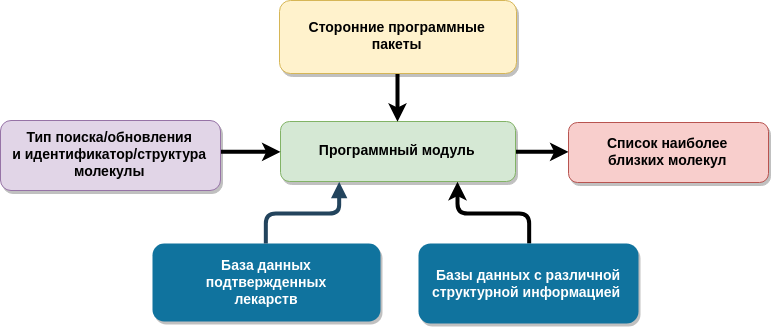
\includegraphics[width=1.0\linewidth]{Drawio/3}} % Вставляем рисунок в полученное "окно" полностью - 100%
		\label{structure}
	\end{minipage}
\end{figure}

\subsection{Материалы и методы исследования}
\subsubsection{Биологические базы данных}
\color{orange} Описание устройства баз и примеры: Drugbank \cite{drugbank}, Uniprot \cite{uniprot} , PDB \cite{pdb}, Pubchem \cite{pubchem}. \color{black}
\subsubsection{Коэффициенты Жаккара и Танимото}
Для удобства работы с мерами сходства как с числами имеет смысл ввести единообразное для самых разных типов данных определение бинарного коэффициента сходства. Коэффициент Жаккара \cite{Jaccard1901} позволяет для любых двух конечных множеств $A, B$ получить коэффициент подобия $J(A, B)$ по формуле
\begin{equation}
\label{jaccard}
J(A, B) = \frac{|A\cap B|}{|A\cup B|} \in [0, 1].
\end{equation}
Видно, что равенство коэффициента нулю означает полное отсутствие сходства между множествами. Чем больше значение $J(A, B)$, тем выше степень сходства множеств вплоть до полного совпадения при $J(A, B) = 1$.

Частным случаем этого коэффициента является коэффициент Танимото, применяющийся в случае сравнения бинарных множеств. Тогда их можно охарактеризовать битовыми векторами $\textbf{a}, \textbf{b}$, а (\ref{jaccard}) можно переписать проще для прямого вычисления:
\begin{equation}
T(\textbf{a}, \textbf{b}) = \frac{\textbf{a}\cdot\textbf{b}}{|\textbf{a}|^2 + |\textbf{b}|^2 - \textbf{a}\cdot\textbf{b}}.
\end{equation}

\subsubsection{Сходство белков по аминокислотной последовательности}
Для вычисления сходства белков по их аминокислотным последовательностям был использован модуль Biopython \cite{biopython}. Он позволяет вычислить подобие и идентичность (\color{orange} ОПРЕДЕЛЕНИЯ \color{black}) двух а/к последовательностей (АКП).(\color{orange} КАК РАБОТАЕТ \color{black}) (\color{orange} ПРИМЕР выравнивания листингом \color{black}) 

\subsubsection{Сходство белков по структуре}
Для вычисления сходства белков, используя их структуру, использована программа TM-align \cite{TM, TMalign}. 
Сначала с помощью динамического программирования определяется оптимальное наложение двух белков друг на друга, которое, вообще, является NP-трудной задачей \cite{Lathrop1994} 
и потому требует существенных вычислительных ресурсов. После этого вычисляется TM-score (англ. Template Modeling score)\cite{Levitt1998} 
\begin{equation}
\label{tm-score}
\text{TM-score} = \max\left[\frac{1}{L_{target}}\sum_i^{L_{aligned}}\frac{1}{1+\left(\frac{d_i}{d_0(L_{target})}\right)^2}\right],
\end{equation}
где $L_{target}$~--- количество а/к в целевом белке, сравниваемом с другими; $L_{aligned}$~--- количество а/к в выравненной части двух белков, $d_i$~--- расстояние между $i$-й парой остатков в белках; $d_0$~--- нормировочный коэффициент $d_0(L_{target}) = 1.24\sqrt[3]{L_{target}-15}-1.8$; сумма производится по парам соответствующих оснований. TM-score нормирован таким образом, что его значение меньше 0,2 говорит об отсутствии корреляций в структурах, а превышение эмпирической границы в 0,5 означает, что укладки белков практически совпадают \cite{TMalign}. 

Одновременно считается и коэффициент RMSD (англ. Root Mean Square Deviation) %\ref{rmsd}
\begin{equation}
\label{rmsd}
\text{RMSD} = \sqrt{\frac{1}{N}\sum_{i=1}^N \delta_i},
\end{equation}
где $N$~--- количество атомов в молекуле; $\delta_i$~--- отклонение $i$-го атома от второй структуры.

TM-score считается более подходящим для оценки подобия белков, чем RMSD, так как в отличие от RMSD он не зависит от длин сравниваемых белков (нормируется на полусумму их длин и находится в полуинтервале $(0, 1]$), а также учитывает различные области белков с разными весами, что позволяет получать адекватные результаты для структур с одинаковой глобальной топологией, но небольшими отклонениями по всей длине белка. В случае использования RMSD результат будет подразумевать то, что структуры различны, а TM-score, вероятнее всего, детектирует схожесть \cite{TMalign}.
\subsubsection{Сходство лигандов по структуре}
Для нахождения сходства лигандов по их топологической структуре могут использоваться молекулярные отпечатки нескольких типов. Существуют различные принципы  построения отпечатков: могут хэшироваться различные топологические пути, могут искаться фармакофоры или определенные подструктуры, существуют и способы с использованием только текста SMILES \cite{Cereto-Massague2015}. Получающиеся битовые строки двух сравниваются, что приводит к коэффициенту Танимото как оценке степени подобия структур.

Мы использовали вычисление таких отпечатков по SMILES (текстовый отпечаток) и SDF файлу (топологические пути). Нахождение этих отпечатков реализовано,  с помощью модулей RDkit \cite{rdkit} и Open Babel \cite{openbabel} соответственно. \sic{Не представляет сложности при необходимости добавить другие типы, например, из тех же модулей.}

\subsubsection{Сходство сайтов связывания}
Для вычисления подобия сайтов связывания используется программный пакет IsoMIF \cite{isomif, Chartier2015}, считающийся одним из лучших для данного вычисления \cite{Ehrt2016}. (\color{orange} ТОЧНО??? Проверить\color{black})

Суть его работы состоит в нахождении полостей структуры комплекса лиганд-мишень\cite{Gaudreault2015, Laskowski1995}(\color{orange} подробнее как ищутся \color{black}). 

После этого с помощью встроенной в пакет программы MIF (англ. Molecular Interaction Field) в области сайта связывания строится сетка, в каждом узле которой считаются энергии взаимодействия пробника определенного типа с соседними атомами белка до некоторого радиуса обрезки. Всего используется 6 типов свойств пробника: гидрофобность, ароматичность, способность быть донором/акцептором водородной связи, положительный/отрицательный электрический заряд, энергии спадают одинаково и экспоненциально от расстояния, а значения энергий на 1 \AA $\:$ подбираются эмпирически для всевозможных пар из 6 типов пробника и 13 видов атома белка (см. рис. \ref{cleft_mif} (б)).

После получения этих сеток для двух сайтов связывания (с 6 значениями энергии в каждом узле) происходит построение графа, у которого вершины обозначают пары узлов сетки, берущихся по одному из сравниваемых структур и имеющих хотя бы один общий из 6 типов энергии больше некоторого порога, то есть является значимым. Ребра в этом графе строятся, если расстояния между соответствующими узлами в двух полостях отличаются менее, чем на 3 \AA. 

Затем в этом графе производится поиск наибольшей клики (полного подграфа) с помощью алгоритма Брона — Кербоша \cite{Bron1973, Tomita2006} и с использованием эвристического наблюдения, что наибольшая клика часто находится одной из первых, так что для значительного уменьшения вычислительной нагрузки проводится только 100 поисков по умолчанию. 

Результат работы алгоритма~--- мера подобия полостей,~--- вычисляется как
\begin{equation}
\text{MSS} = \frac{N_c}{N_a + N_b - N_c},
\end{equation} \cite{Chartier2015}.
где $N_c$~--- количество значимых общих типов взаимодействий у всех вершин в клике, $N_a, N_b$~--- количества значимых типов взаимодействий в узлах сеток для первого и второго белка. 

\color{orange} TM-align?\color{black}
\begin{figure} 
	\caption{Визуализация работы (а) поиска полостей и (б) вычисления MIF(\color{orange} сделать картинки одного формата \color{black})} 
	\label{cleft_mif} 
	\begin{subfigure}{.45\textwidth}
		\centering
		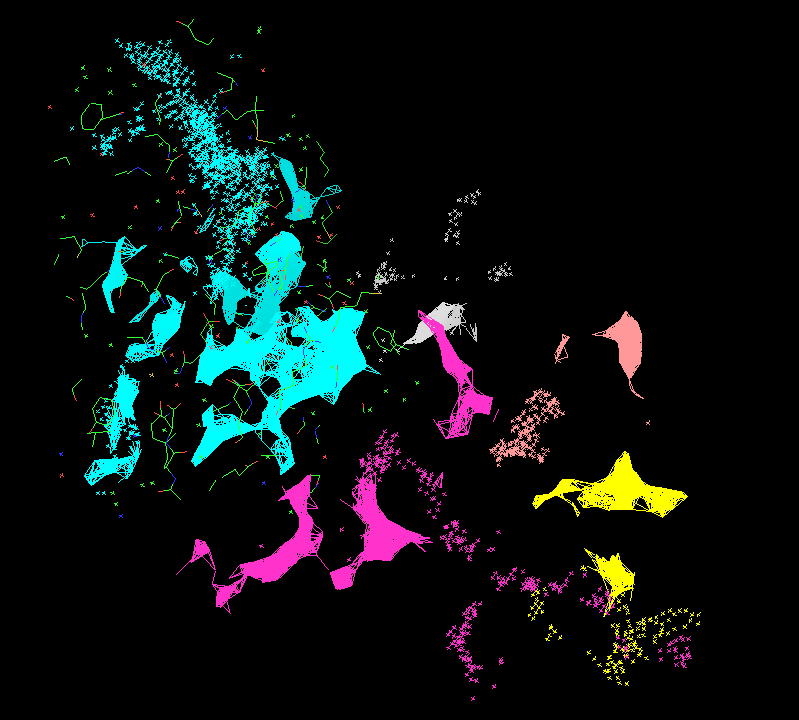
\includegraphics[width=1\linewidth]{pictures/clefts}
		\caption{Пять наибольших найденных с помощью Get Cleft полостей комплекса показаны разными цветами.}
		\label{fig:sfig1}
	\end{subfigure}
	\hfill
	\begin{subfigure}{.45\textwidth}
		\centering
		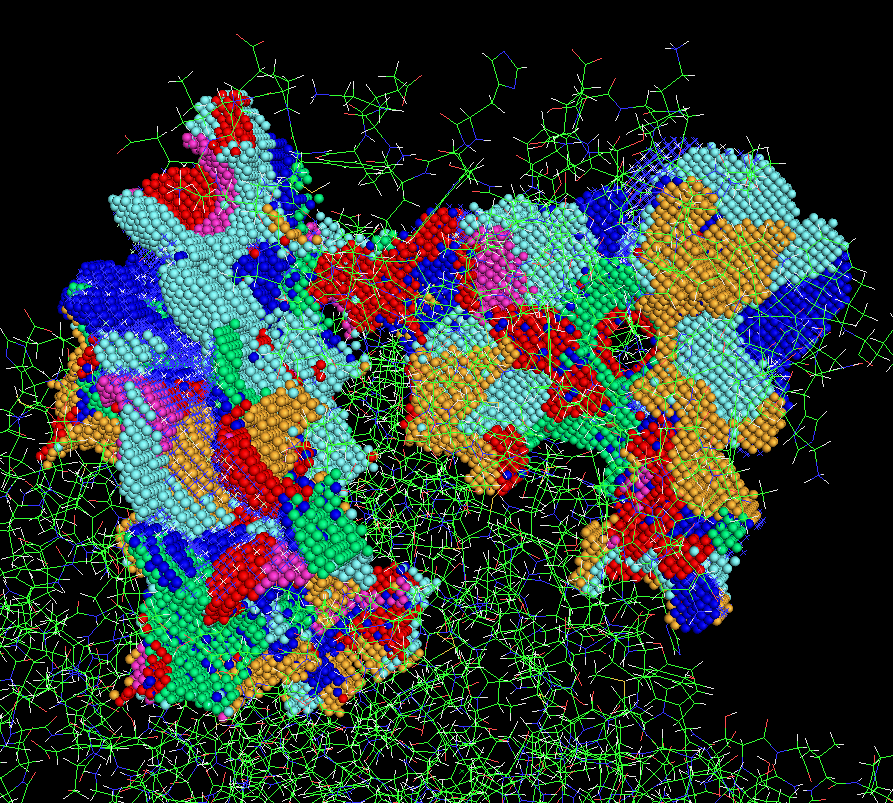
\includegraphics[width=1\linewidth]{pictures/mif}
		\caption{Размеченная посредством MIF полость, разные цвета обозначают тип максимального по энергии взаимодействия в этой области.}
		\label{fig:sfig2}
	\end{subfigure}
\end{figure}
\newpage
\subsection{Описание программного модуля и результаты}
Программный код на языке программирования Python 3.7 \cite{python37} и содержащий более ?1000 строк доступен в открытом репозитории \linebreak \href{https://github.com/antmaxi/BSc\_thesis}{https://github.com/antmaxi/BSc\_thesis}.

Модуль состоит из четырех программ: Search.py, Drugbank.py, IsoMIF.py, Auxiliary.py, различные функции из которых могут вызываться посредством вызова программы Search.py с соответствующими потребностям пользователя или другой программы ключами. \color{orange} ключи еще не сделаны \color{black}

Состав программ:
\begin{enumerate}
	\item Search.py~--- все, кроме реализованной с помощью программного пакета IsoMIF, функции обработки данных для получения значений метрик схожести и скрининга по референсным данным.
	\item Drugbank.py~--- функции для извлечения, дополнения и обработки референсных данных из БД Drugbank.
	\item IsoMIF.py~--- функции для проведения поиска схожих комплексов с помощью IsoMIF.
	\item Auxiliary.py~--- вспомогательные функции для работы с файловой системой, для соединения записей об одной молекуле с помощью ID различных БД (Drugbank, PubChem, Uniprot, PDB) и разных характеристик (SMILES, а/а последовательность).
\end{enumerate}

Работа модуля была протестирована на компьютере с операционной системой Ubuntu 16.04 LTS 64-bit, с процессором Intel® Core™ i9-7940X CPU @ 3.10GHz $\times$ 28 и видеокартой GeForce GTX 1080 Ti/PCIe/SSE2.
\subsubsection{Извлечение данных}
Было решено производить извлечение референсных данных из БД Drugbank, так как она является наиболее полной и хорошо аннотированной БД лекарств \sic{cite{}} и содержит не только информацию о лигандах, но и о мишенях вместе со ссылками на другие специфические источники информации. 

Хотя в приложении к полной БД Drugbank находятся таблицы с частью нужной для работы протокола информации (ссылки на другие БД, химические идентификаторы), было принято решение извлекать информацию напрямую из полной БД, что позволяет: 

(а) не зависеть от обновления приложений ко всей БД, которые могут запаздывать относительно общего обновления БД; 

(б) делать поиск по нужным записям/свойствам более гибким и простым для будущих модификаций и усовершенствований протокола.

\subsubsection{Сходство белков по аминокислотной последовательности}

В цикле по мишеням, извлеченным из БД Drugbank, производится сравнение АКП входного белка (можно задать по последовательности или ID Uniprot, тогда АКП запрашивается у онлайн-сервиса Uniprot) с АКП соответствующей мишени. Результатом каждого сравнения является пара чисел (подобие, идентичность), характеризующих степень похожести АКП. Затем производится сортировка полученного списка по одной из этих мер подобия, и результат выводится на экран.

Пример использования этой функции в листинге \ref{lst:fasta}
\color{black}. Была взята АКП GPCR человеческого белка родопсина, одного из важнейших белков у человека и ключевого инструмента оптогенетики. Неудивительно, что наиболее похожей мишенью из БД Drugbank оказался он же сам. Последовательности остальных найденных белков сильно отличаются от данной (падение схожести с 1843 до 318, идентичности с 348 до 156), \sic{Почему нет GPCR?} так что, вероятно, в данном случае сложно говорить о возможности совпадения лигандов родопсина и остальных мишеней из списка.
\begin{lstlisting}[language=Python, label={lst:fasta}, caption={Определение сходства мишеней по а/к последовательности посредством Biopython, входные данные~--- ID Uniptor человеческого родопсина из семейства GPCR.}]
In:
	get_closest_fastas_from_uniprot('P08100', path_to_data_in_fasta, k=0, align_matrix='blosum62', sim_or_ident=True)
Out:

	 	position_in_fasta 	similarity 	identity 	sequence 	name
	1392 	 	1392 	1843 	348  	lcl|BSEQ0016346|Rhodopsin
	1931 	 	1931 	318 	156 	lcl|BSEQ0010278|Cholecystokinin
	151 	 	151 	295 	147 		lcl|BSEQ0016698|Somatostatin
	152 	 	152 	292 	154 		lcl|BSEQ0006800|Somatostatin
	676 	 	676 	270 	156 	lcl|BSEQ0002303|Gastrin/cholecystokinin
	1317 	 	1317 	262 	139 	lcl|BSEQ0010362|Melatonin
	711 	 	711 	250 	147 		lcl|BSEQ0001536|Mu-type

CPU times: user 10min 41s, sys: 1.26 s, total: 10min 42s
Wall time: 10min 43s
\end{lstlisting}
Сравнение одной пары занимает от долей секунды до около 10 секунд, вся база данных порядка 10-30 минут.
\subsubsection{Сходство белков по структуре}
Список ID PDB, в которые входит белок, автоматически берется с помощью онлайн~-сервиса БД Unirprot. Далее необходимо из этих структур выбрать те, в которых белок находится сам по себе, без других аминокислотных цепей (так как TM-align считает схожесть для всех атомов в аминокислотах, даже если белков или их частей в файле несколько)

Для такой фильтрации списка используется ранее упоминавшееся вычисление схожести а/к последовательностей. .....
\color{orange} В ПРОЦЕССЕ, КОД ПИШУ
\color{black}
\subsubsection{Сходство лигандов по структуре}
\color{orange} ОТНОСИТЕЛЬНО ПОДРОБНО РАСПИСАНО, ТАК ВСЕ БУДУТ ТИПЫ ПОИСКОВ (+КАРТИНКИ НАДО)
\color{black}

Поиск по ID SMILES:

Из БД Drugbank извлекаются соответствующие ID SMILES подтвержденных FDA лигандов. Информация дополняется извлеченными из БД PubChem (\href{https://pubchem.ncbi.nlm.nih.gov}{https://pubchem.ncbi.nlm.nih.gov}) идентификаторами тех лигандов, у которых нет ID SMILES в БД Drugbank, но имеющих запись в БД PubChem.

Далее, с помощью ПМ RDkit строятся и сравниваются молекулярные отпечатки, вычисляется коэффициент Танимото между ними, приводя к отсортированному по степени подобия списку подтвержденных FDA лигандов. Пример приведен в листинге \ref{lst:smiles-fing}.

\begin{lstlisting}[language=Python, label={lst:smiles-fing}, caption={Сходство лигандов по текстовым молекулярным отпечаткам с помощью ПМ RDkit для входных данных~--- SMILES структуры молекулы}]
In:
	get_closest_smiles_names('ClCCNC(=O)N(CCCl)N=O', root, 5)
Out:
	query       			smiles  						similarity         			 name
	124   O=NN(CCCl)C(=O)NCCCl      ClCCNC(=O)N(CCCl)N=O    1.000000    Carmustine
	919   O=NN(CCCl)C(=O)NCCCl  ClCCN(N=O)C(=O)NC1CCCCC1    0.644351     Lomustine
	465   O=NN(CCCl)C(=O)NCCCl            NCC=C.ClCC1CO1    0.550000     Sevelamer
	1110  O=NN(CCCl)C(=O)NCCCl              NC(CO)(CO)CO    0.540984  Tromethamine
	1066  O=NN(CCCl)C(=O)NCCCl                 CCCCCON=O    0.524590  Amyl Nitrite
CPU times: user 2.66 s, sys: 7.99 ms, total: 2.67 s
Wall time: 2.66 s
\end{lstlisting}

Поиск по структуре в формате SDF:

С сайта БД Drugbank скачивается файл со структурами всех лигандов в формате SDF, из него по ID в БД Drugbank извлекаются структуры подтвержденных FDA лигандов. Затем по этим структурам получаются молекулярные отпечатки, вычисляется коэффициент Танимото между ними, результируя в искомом списке. Пример приведен в листинге \ref{lst:sdf-fing}.

\begin{lstlisting}[language=Python, label={lst:sdf-fing}, caption={Сходство лигандов по топологическим молекулярным отпечаткам с помощью ПМ Open Babel для входных данных~--- SDF структуры молекулы}]
In: 
	get_closest_ligands_from_3d_structure(path_to_structure, path_to_sdf_approved, root,
fptype='maccs', number_to_print=5)
Out:
Name  				Tanimoto coeff 	Drugbank ID 	Fingerprint_type
0  Dichlorobenzyl alcohol        0.343284     DB13269              fp2
1         Tiludronic acid        0.317647     DB01133              fp2
2           Chloroxylenol        0.308824     DB11121              fp2
3             Sulconazole        0.290598     DB06820              fp2
4               Guanabenz        0.268293     DB00629              fp2
CPU times: user 1.87 s, sys: 7.68 ms, total: 1.88 s
Wall time: 1.88 s
\end{lstlisting}
\color{orange} НУЖНО ЛИ ПОДРОБНО ОБЪЯСНЯТЬ, ЧТО ВВОДИТСЯ, ЧТО ВЫВОДИТСЯ?
\color{black}
\color{orange} КАРТИНКА СО СРАВНЕНИЕМ ИЗОБРАЖЕНИЙ МОЛЕКУЛ
\color{black}

Время поиска по фармакофорам 1-3 сек.
\subsubsection{Сходство сайтов связывания}
Для сравнения комплекса из входных данных с референсными комплексами необходимо каким-то образом получить их структуры. С этой целью для лиганда и мишени строятся два списка ID PDB, включающих в себя их. 

Для мишени список составляется просто по ID Uniprot c помощью запросов к онлайн~-сервису БД Uniprot, позволяющего находить соответствующие данному белку ID PDB (при этом может случиться, что в этих структурах находится белок как сам по себе, так и в комплексе с некоторым лигандом). 

Для лиганда по его SMILES ищутся ID PDB, в которых есть похожая на него структура. Для этого нужно ввести требуемый уровень коэффициента Танимото или же указать шаг, с которым этот коэффициент будет уменьшаться начиная с 1 до тех пор, пока не будет найдена хотя бы одна структура в БД PDB.

Затем находятся общие элементы списков ID PDB для мишени и лиганда. Из них можно взять тот, с которым подобие лиганда максимально для ускоренного поиска, или же использовать все.

В конце концов, с помощью ПМ IsoMIF находятся коэффициент подобия карманов связывания для всех найденных референсных структур комплексов и входного комплекса, и выводятся наиболее похожие.

Для одной пары полостей время построения MIF обычно около 1--3 мин, время вычисления IsoMIF около 3--5 мин, остальные части этого поиска длятся пренебрежимо мало.

Возможно, в будущем для ускорения работы стоит сделать параллельную версию этой части протокола.

\newpage
\section{Заключение}
Построен протокол поиска подобных и соответствующих подтвержденным FDA лигандов/мишеней/комплексов по нескольким типам входных данных с использованием различных способов задания вычисления подобия: по 1D\,--, 2D\,--, 3D\,--\,структурам. Работа протокола проверена и задокументирована, программный код и примеры опубликованы в открытом доступе. (\color{orange} В ПРОЦЕССЕ \color{black})

Из-за своей модульной структуры в будущем протокол может дополняться новыми вариантами нахождения меры схожести. Также на его основе с применением машинного обучения могут быть построены более сложные методы поиска, учитывающие несколько различных метрик подобия.


\newpage
%\section{}
\printbibliography[heading=bibintoc, title=Список использованных источников]

\end{document}